% Manuscript prepared with the LLNCS macro package (Springer).
% Version 2.21 of 2022/01/12
%
\documentclass[runningheads]{llncs}
%
\usepackage[T1]{fontenc}
\usepackage{graphicx}
\usepackage{amssymb}
\usepackage{amsmath}
\usepackage{booktabs}
\usepackage{xurl}
\usepackage{hyperref}
\usepackage{enumitem}
\usepackage{tikz}
\usetikzlibrary{arrows.meta,positioning,fit,calc,shapes.misc,backgrounds}

\title{An Empirical Assessment of DQN-Based Centrality Selection for Matrix Bandwidth Minimization}
\titlerunning{Empirical Assessment of DQN-Based Centrality Selection}
\author{Anonymous Authors}
\date{}

\begin{document}
\maketitle

\begin{abstract}
The Matrix Bandwidth Minimization Problem (MBMP) seeks vertex orderings that reduce the maximum distance of nonzero entries from the main diagonal of a sparse matrix. This paper evaluates a Deep Q-Network (DQN) selection hyper-heuristic that chooses among seven graph-centrality-based constructive heuristics. Experiments on 13 benchmark instances with 30 seeds and matched constructive-search budgets compare DQN with uniform random selection, all seven fixed centralities, a per-instance virtual best solver (VBS), a single best solver (SBS), and Reverse Cuthill--McKee (RCM). The DQN does not consistently outperform random selection or the strongest fixed centralities and closes only 2.2\% of the normalized SBS--VBS gap. A $2\times2$ ablation crossing \{DQN, Random\} with \{centrality-based, pseudo-peripheral\} initialization shows that pseudo-peripheral starts improve all six LSHP instances by 2.7--4.4\% for DQN, with a similar effect under Random selection, while degrading BCS, BP, and SHL cases. Under pseudo-peripheral initialization, DQN and Random are not significantly different on any tested instance. These results indicate that the main observed gains arise from family-dependent constructive-search choices rather than from the learned selector itself.
\end{abstract}

\noindent\textbf{Keywords:} Matrix bandwidth minimization; deep reinforcement learning; hyper-heuristics; graph centrality; sparse matrices.
\section{Introduction}

The ordering of rows and columns in sparse matrices affects storage and the computational behavior of sparse linear algebra routines. Bandwidth reduction seeks to place nonzero coefficients near the main diagonal. In graph terms, matrix rows and columns correspond to vertices, off-diagonal nonzeros to edges, and a permutation to a vertex labeling.

The Matrix Bandwidth Minimization Problem (MBMP) is computationally difficult and has motivated numerous heuristics, including Cuthill--McKee, Reverse Cuthill--McKee (RCM), and several metaheuristics. However, no single low-cost heuristic consistently dominates across different graph families and matrix structures \cite{gonzaga2025}. This variability motivates adaptive approaches that select search strategies according to the current search context.

Selection hyper-heuristics address this problem by choosing among low-level heuristics rather than searching directly in the solution space \cite{burke2013}. Reinforcement learning (RL), particularly deep RL, has become an important mechanism for adaptive heuristic selection in combinatorial optimization \cite{mazyavkina2021,kallestad2023,zhang2022}. In this setting, an RL agent can learn which low-level heuristic is more promising for a given search state.

Building on previous multi-centrality reinforcement-learning approaches, this work develops and systematically evaluates a DQN-based selection hyper-heuristic for MBMP. The agent selects among seven graph-centrality measures, each guiding a randomized constructive heuristic that generates candidate orderings. The main question is whether learned adaptive selection provides an advantage over fixed and random centrality-selection strategies under equivalent search budgets.

The contributions are a seven-action DQN hyper-heuristic with a normalized state and stabilized training, together with a matched-budget evaluation using 30 seeds per instance against fixed centralities, uniform random selection, a virtual best single heuristic, and RCM. The focus is whether learned selection adds measurable value beyond diversification under equivalent computational conditions.

\section{Background and Related Work}

\subsection{Matrix Bandwidth Minimization}

Let $G=(V,E)$ be an undirected graph associated with a sparse symmetric matrix, and let
\[
\pi: V \rightarrow \{1,\ldots,|V|\}
\]
be a bijective vertex labeling. The bandwidth induced by $\pi$ is
\[
B(G,\pi)=\max_{(u,v)\in E} |\pi(u)-\pi(v)|.
\]
The MBMP consists of finding
\[
\pi^\star = \arg\min_{\pi} B(G,\pi).
\]

Classical bandwidth-reduction methods include the Cuthill--McKee ordering \cite{cuthill1969} and its reverse variant, which are widely used because of their low computational cost. Nevertheless, the quality of such methods varies across graph classes and matrix structures. Gonzaga de Oliveira \cite{gonzaga2025} provides a recent overview of heuristics and metaheuristic strategies for matrix bandwidth reduction.

\subsection{From Dynamic Programming to Reinforcement Learning}

Reinforcement learning models sequential decisions in which an agent interacts with an environment to maximize cumulative reward, with roots in dynamic programming and Bellman's principle of optimality \cite{bellman1957}. A Markov Decision Process is commonly represented by
\[
\mathcal{M}=(\mathcal{S},\mathcal{A},P,R,\gamma),
\]
where $\mathcal{S}$ and $\mathcal{A}$ are the state and action spaces, $P$ the transition model, $R$ the reward, and $\gamma$ the discount factor.

Q-learning \cite{watkins1992} is a model-free off-policy method with update
\[
Q(s_t,a_t)\leftarrow Q(s_t,a_t)+
\eta\left[
r_{t+1}+\gamma\max_{a'}Q(s_{t+1},a')-Q(s_t,a_t)
\right].
\]
For large or continuous state spaces, Deep Q-Networks replace the Q-table with a neural network $Q(s,a;\theta)$ \cite{mnih2015}. The network approximates Bellman targets, while $\epsilon$-greedy exploration balances random actions and greedy choices. Replay memory and a separate target network are commonly used to stabilize learning. These components are instantiated explicitly in Section~3.

\subsection{Reinforcement Learning as a Hyper-Heuristic}

Selection hyper-heuristics operate above problem-specific heuristics by choosing among low-level methods according to the current search context \cite{burke2013}. This is attractive when different heuristics perform well on different instances or search stages. Deep RL has increasingly been used for combinatorial optimization and adaptive heuristic selection \cite{mazyavkina2021,zhang2022,kallestad2023}. In the present formulation, the DQN does not construct a permutation directly; its action selects a graph-centrality measure that guides a randomized constructive procedure. Learning therefore acts as an adaptive decision layer over problem-specific heuristics.

\subsection{Relation to the Previous Q-MCH Study}

The Q-MCH approach of Carneiro et al.~\cite{carneiro2024qmch} directly precedes this work by combining a DQN with a multi-centrality constructive heuristic for matrix bandwidth reduction. The present study extends that formulation from two to seven centrality actions and introduces a normalized 12-dimensional state, a dense reward, replay memory, a target network, terminal-state masking, gradient clipping, and controlled exploration.

More importantly, the experimental question is different. Rather than asking only whether reinforcement-learning-guided multi-centrality search can improve classical baselines, we assess whether the learned selector itself provides value beyond random diversification and fixed centrality choices under matched search budgets. The evaluation therefore includes all seven fixed centralities, a virtual best single heuristic (VBS), and paired experiments over 30 seeds. The results provide a controlled assessment of both the value and the limitations of reinforcement learning for centrality selection.

\section{Proposed Method}

\subsection{Overview}

The proposed approach treats centrality selection as a sequential decision problem. Before training, the input matrix is converted into an undirected graph and seven centrality maps are computed once. At each search step, the DQN receives a normalized state containing search progress, current and incumbent bandwidth information, stagnation, and the observed success rate of each available action. The selected centrality guides a randomized constructive heuristic that evaluates 15 candidate constructions. The best candidate obtained for that action is then used to compute a dense reward and update the search state. Figure~\ref{fig:framework} summarizes the complete interaction loop.



\begin{figure*}[t]
\centering

\resizebox{\textwidth}{!}{%
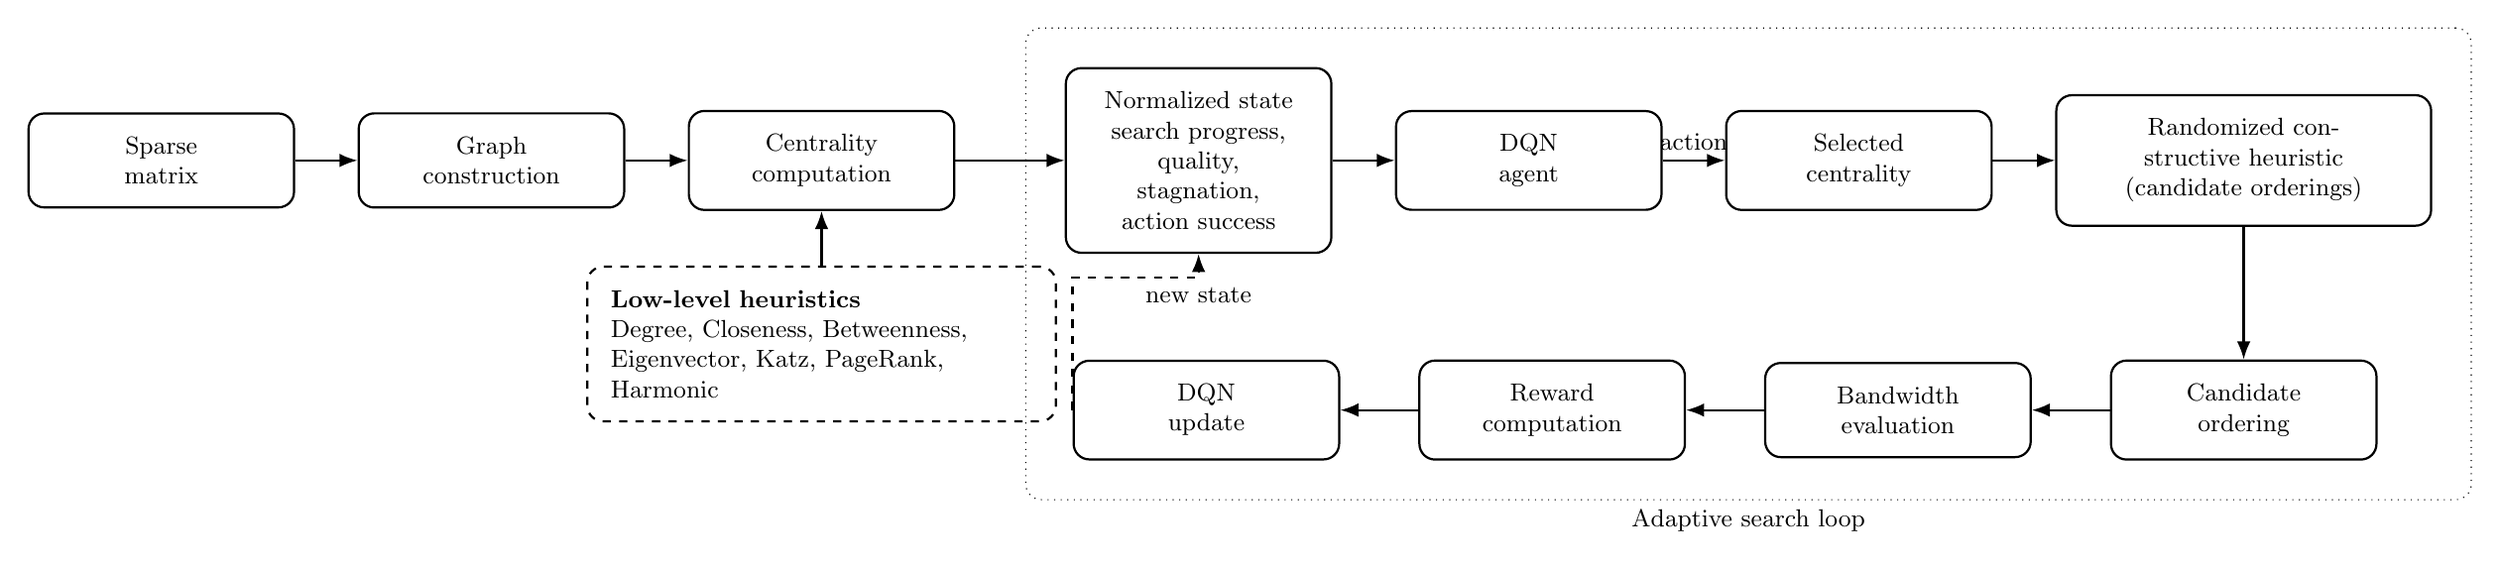
\begin{tikzpicture}[
    font=\small,
    >=Latex,
    box/.style={
        draw,
        rounded corners=2mm,
        thick,
        align=center,
        minimum height=9mm,
        text width=2.8cm,
        inner sep=3mm
    },
    widebox/.style={
        draw,
        rounded corners=2mm,
        thick,
        align=center,
        minimum height=10mm,
        text width=4.2cm,
        inner sep=3mm
    },
    pool/.style={
        draw,
        rounded corners=2mm,
        dashed,
        thick,
        align=left,
        text width=5.4cm,
        inner sep=3mm
    },
    line/.style={->, thick},
    feedback/.style={->, thick, dashed}
]

% Top pipeline
\node[box] (matrix) {Sparse\\matrix};
\node[box, right=8mm of matrix] (graph) {Graph\\construction};
\node[box, right=8mm of graph] (centcomp) {Centrality\\computation};

\node[pool, below=7mm of centcomp] (pool) {
\textbf{Low-level heuristics}\\
Degree, Closeness, Betweenness,\\
Eigenvector, Katz, PageRank,\\
Harmonic
};

\node[box, right=14mm of centcomp] (state) {
Normalized state\\
search progress, quality,\\
stagnation, action success
};

\node[box, right=8mm of state] (dqn) {DQN\\agent};
\node[box, right=8mm of dqn] (action) {Selected\\centrality};

\node[widebox, right=8mm of action] (construct) {
Randomized constructive heuristic\\
(candidate orderings)
};

% Bottom pipeline
\node[box, below=17mm of construct] (ordering) {
Candidate\\ordering
};

\node[box, left=10mm of ordering] (bandwidth) {
Bandwidth\\evaluation
};

\node[box, left=10mm of bandwidth] (reward) {
Reward\\computation
};

\node[box, left=10mm of reward] (update) {
DQN\\update
};

% arrows top
\draw[line] (matrix) -- (graph);
\draw[line] (graph) -- (centcomp);
\draw[line] (centcomp) -- (state);
\draw[line] (state) -- (dqn);

\draw[line] (dqn) --
node[above, sloped] {action}
(action);

\draw[line] (action) -- (construct);

% pool link
\draw[line] (pool.north) -- (centcomp.south);

% down to bottom
\draw[line] (construct) -- (ordering);
\draw[line] (ordering) -- (bandwidth);
\draw[line] (bandwidth) -- (reward);
\draw[line] (reward) -- (update);

% feedback to state
\draw[feedback]
(update.west)
|- ($(state.south)+(0,-3mm)$)
-| node[pos=0.25, below] {new state}
(state.south);

% Background grouping
\begin{scope}[on background layer]

\node[
    draw,
    rounded corners=2mm,
    dotted,
    inner sep=5mm,
    fit=(state)(dqn)(action)(construct)
        (ordering)(bandwidth)(reward)(update),
    label={[font=\small]below:Adaptive search loop}
] {};

\end{scope}

\end{tikzpicture}%
}

\caption{
DQN-based adaptive centrality selection framework for matrix bandwidth minimization, where the agent selects a centrality from a compact state and receives reward based on the bandwidth improvement achieved by the constructive search.
}
\label{fig:framework}

\end{figure*}

%The overall process is:
%\begin{enumerate}
 %   \item convert the sparse matrix into an undirected graph;
  %  \item compute the seven centrality maps;
  %  \item initialize the incumbent with the bandwidth of the original ordering;
  %  \item let the DQN select one of the seven centralities;
  %  \item generate 15 candidate constructions using the selected centrality;
  %  \item retain the best candidate bandwidth returned by that action;
  %  \item update the incumbent when an improvement is found;
  %  \item compute the dense reward and update the normalized state;
   % \item store the transition in replay memory and update the online network;
   % \item periodically synchronize the target network;
   % \item repeat for 300 training decisions and then evaluate the frozen greedy policy for 60 additional decisions.
%\end{enumerate}

\subsection{Low-Level Heuristics}

The action set contains seven centralities: Degree, Closeness, Betweenness, Eigenvector, Katz, PageRank, and Harmonic centrality. For a selected centrality $c$, the constructive procedure uses a randomized restricted candidate list with $\alpha_{\mathrm{RCL}}=0.3$. Vertices within each breadth-first level are sorted according to the selected centrality; the top $\alpha_{\mathrm{RCL}}$ fraction forms the restricted set, after which both the restricted and complementary sets are independently shuffled before concatenation. This preserves a centrality-guided preference while generating different orderings across repeated constructions.

In the main formulation, the initial vertex is sampled with probability proportional to the selected centrality values. If the resulting weights are invalid---for example, because they are non-finite, negative, or have zero total mass---the implementation falls back to uniform sampling. The remaining labeling is then constructed level by level through a breadth-first traversal.

At each DQN decision, the selected low-level heuristic performs 15 randomized constructions and returns the best bandwidth found. The same number of constructions per decision is used by the matched random and fixed-centrality baselines. A separate structural ablation, reported in Section~\ref{sec:peripheral}, replaces centrality-weighted initial-vertex sampling with a pseudo-peripheral starting vertex while retaining centrality-guided ordering within the BFS levels.

\subsection{State Representation}

The DQN uses a normalized 12-dimensional state vector:
\[
s_t =
\left[
\frac{t}{T},
\frac{B_t}{B_0},
\frac{B_t^\star}{B_0},
\frac{B_0-B_t^\star}{B_0},
\frac{\tau_t}{T},
\rho_{1,t},\ldots,\rho_{7,t}
\right],
\]
where $T$ is the training horizon, $B_0$ is the initial bandwidth, $B_t$ is the bandwidth returned by the most recent selected heuristic, $B_t^\star$ is the best bandwidth found so far, and $\tau_t$ is the number of decisions since the last strict incumbent improvement. For action $i$, $\rho_{i,t}$ is the empirical strict-improvement rate, defined as the number of times action $i$ improved the incumbent divided by the number of times it was selected up to decision $t$.

The normalization removes bandwidth-scale dependence and summarizes search progress, stagnation, and action effectiveness, but does not encode graph topology.

\subsection{Reward Function}

A dense reward is used to provide feedback even when a newly generated candidate does not improve the incumbent. Let $B^\star_{t-1}$ be the incumbent bandwidth before action $a_t$, let $B_t$ be the candidate returned by the selected heuristic, and let $B_0$ be the initial bandwidth. The reward is
\[
r_t =
\begin{cases}
\dfrac{B^\star_{t-1}-B_t}{B_0}, & B_t < B^\star_{t-1},\\[7pt]
0.01, & B_t = B^\star_{t-1},\\[5pt]
-0.05\min\!\left(\dfrac{B_t-B^\star_{t-1}}{B_0},1\right), & B_t > B^\star_{t-1}.
\end{cases}
\]

Thus, improvements receive a reward proportional to their normalized magnitude, ties receive a small positive signal, and deteriorations are mildly penalized. This design is intended to reduce reward sparsity while keeping incumbent improvement as the primary objective.

\subsection{DQN Architecture and Learning}

The online Q-network contains two fully connected hidden layers with 128 neurons each and ReLU activations. The output layer contains seven Q-values, one for each centrality action. A separate target network is maintained to stabilize Bellman updates.

The main hyperparameters are $\eta = 0.001$, $\gamma = 0.9$, $\epsilon_0 = 1.0$, and $\epsilon_{\min}=0.01$. Exploration follows the exponential schedule
\[
\epsilon_t=\max\!\left(\epsilon_{\min},
\epsilon_0\left(\frac{\epsilon_{\min}}{\epsilon_0}\right)^{t/T}\right),
\]
with $T=300$. During the subsequent 60-decision evaluation phase, the network is frozen and the policy acts greedily.

Transitions are stored in a replay buffer with capacity 10,000. Learning starts when 64 transitions are available and uses mini-batches of size 64. The target network is synchronized every 25 gradient updates. The Bellman target is
\[
y_t = r_t + \gamma (1-d_t)\max_a Q_{\mathrm{target}}(s_{t+1},a),
\]
where $d_t$ indicates a terminal transition. The network is trained with Smooth L1 loss and Adam, and the gradient norm is clipped at 1.0.

Each run contains 300 training and 60 frozen greedy decisions, totaling 5,400 constructive evaluations. With a 64-transition warm-up, training yields 237 gradient updates and nine target-network synchronizations, so the replay buffer is only partially used.

\section{Experimental Setup}

\subsection{Dataset and Instance Origin}

The evaluation uses 13 unique benchmark instances from the Harwell--Boeing benchmark lineage and the HB group of the SuiteSparse Matrix Collection \cite{davis2011,duff1989}: four BCS instances (\texttt{bcsstk01}, \texttt{bcsstk04}, \texttt{bcsstk05}, and \texttt{bcsstk06}), six LSHP instances (\texttt{lshp265}, \texttt{lshp406}, \texttt{lshp1009}, \texttt{lshp1270}, \texttt{lshp1561}, and \texttt{lshp1882}), two BP instances (\texttt{bp\_0} and \texttt{bp\_200}), and one SHL instance (\texttt{shl\_0}). The LSHP matrices correspond to the classical L-shaped problems, whereas BP and SHL are unsymmetric simplex-basis matrices.

All instances are converted into simple undirected graphs. For BP and SHL, the graph uses the union of the sparsity patterns of $A$ and $A^{T}$. Self-loops and duplicate edges are removed, while isolated vertices are preserved.

Two repository files are excluded from the independent-instance analysis. \texttt{bcsstk02} is the complete graph $K_{66}$ in the benchmark representation and therefore has invariant bandwidth 65 under every ordering. In addition, \texttt{bcsstk07.mtx} is byte-identical to the repository copy of \texttt{bcsstk06.mtx} and is not treated as an independent instance.

\subsection{Baselines}

The comparisons are: (i) \textbf{Random}, which selects uniformly among the seven actions; (ii) all seven \textbf{fixed centralities}; (iii) the \textbf{VBS}, defined per instance as the fixed centrality with the lowest mean bandwidth over the 30 runs, after which the 30 runs of that same centrality are reported; (iv) the \textbf{SBS}, the single fixed centrality with the best mean rank across the complete benchmark; and (v) deterministic \textbf{RCM}. The SBS is Katz centrality, with a mean rank of 2.50 when only the seven fixed solvers are considered.

Random and every fixed baseline receive the same 5,400-construction budget as DQN. All stochastic methods start from $B_0$ as incumbent. RCM is reported as its raw bandwidth, not $\min(B_0,B_{\mathrm{RCM}})$.

\subsection{Evaluation Protocol}

All stochastic methods use 30 deterministic seeds. DQN performs 300 training decisions followed by 60 frozen greedy decisions, with 15 constructions per decision. Results are summarized by mean and standard deviation.

Pairwise comparisons centered on DQN use the two-sided Wilcoxon signed-rank test with normal approximation, zero differences removed (\texttt{zero\_method=wilcox}), and no continuity correction. Within each instance, the DQN--Random and DQN--SBS $p$-values are adjusted by Holm's procedure. Global comparisons use the Friedman test with average ranks and tie correction.

To quantify algorithm-selection benefit, we also report the fraction of the SBS--VBS gap closed by DQN,
\[
\mathrm{GapClosed}=\frac{SBS-DQN}{SBS-VBS}.
\]
Because bandwidth scales differ strongly across instances, the benchmark-level score uses the mean normalized bandwidth $B/B_0$ before applying this expression.

\subsection{Computational Environment}

Experiments ran on GitHub Actions (\texttt{ubuntu-24.04}) with CPython 3.11.17, CPU-only PyTorch 2.14.1, NetworkX 3.6.1, NumPy 2.4.6, SciPy 1.17.1, and Pandas 3.0.6. GitHub-hosted runners are dynamically provisioned, so no fixed physical CPU model is assumed.

Because GitHub-hosted runners are dynamically provisioned, wall-clock times are treated as secondary evidence. In the paired $2\times2$ jobs, DQN and Random were executed on the same runner allocation. Averaged over all 300 paired runs, the DQN standard configuration required about 5.4\% more wall-clock time than Random; with pseudo-peripheral initialization the overhead was about 6.2\%. This indicates that network inference and learning add modest overhead relative to the constructive search itself.

\section{Results}

Table~\ref{tab:mainresults} summarizes the 13 instances over 30 seeds. VBS now denotes the best \emph{single fixed centrality per instance}, selected by its 30-run mean rather than by taking a per-seed minimum.

\begin{table*}[t]
\centering
\caption{Main results over 30 seeds. Stochastic methods are reported as mean $\pm$ standard deviation; RCM is deterministic.}
\label{tab:mainresults}
\scriptsize
\begin{tabular}{lrrrrrrr}
\toprule
Instance & $|V|$ & $|E|$ & $B_0$ & RCM & DQN & Random & VBS\\
\midrule
bcsstk01 & 48 & 176 & 35 & 26 & $26.20\pm0.55$ & $26.43\pm0.50$ & $\mathbf{25.83\pm0.65}$\\
bcsstk04 & 132 & 1758 & 47 & 54 & $47.00\pm0.00$ & $47.00\pm0.00$ & $47.00\pm0.00$\\
bcsstk05 & 153 & 1135 & 28 & 24 & $28.00\pm0.00$ & $28.00\pm0.00$ & $28.00\pm0.00$\\
bcsstk06 & 420 & 3720 & 47 & 50 & $47.00\pm0.00$ & $47.00\pm0.00$ & $47.00\pm0.00$\\
bp\_0 & 822 & 3260 & 820 & 422 & $573.43\pm3.20$ & $572.93\pm4.12$ & $\mathbf{572.70\pm3.10}$\\
bp\_200 & 822 & 3788 & 820 & 506 & $600.57\pm4.63$ & $597.30\pm5.29$ & $\mathbf{597.63\pm5.08}$\\
lshp265 & 265 & 744 & 256 & 18 & $25.00\pm0.59$ & $25.00\pm0.64$ & $\mathbf{24.40\pm0.56}$\\
lshp406 & 406 & 1155 & 394 & 22 & $31.37\pm0.56$ & $31.27\pm0.58$ & $\mathbf{30.67\pm0.48}$\\
lshp1009 & 1009 & 2928 & 991 & 34 & $51.23\pm0.57$ & $50.80\pm0.76$ & $\mathbf{50.40\pm0.62}$\\
lshp1270 & 1270 & 3699 & 1250 & 38 & $58.07\pm0.94$ & $57.63\pm0.61$ & $\mathbf{56.93\pm0.52}$\\
lshp1561 & 1561 & 4560 & 1539 & 42 & $64.27\pm0.83$ & $64.27\pm0.83$ & $\mathbf{63.50\pm0.51}$\\
lshp1882 & 1882 & 5511 & 1858 & 46 & $70.93\pm0.91$ & $70.73\pm0.83$ & $\mathbf{70.03\pm0.56}$\\
shl\_0 & 663 & 1682 & 661 & 424 & $493.33\pm9.52$ & $497.80\pm8.09$ & $\mathbf{485.00\pm6.46}$\\
\bottomrule
\end{tabular}
\end{table*}

\subsection{Fixed Centralities, VBS, and SBS}

The best fixed action is instance-dependent: Eigenvector is best on \texttt{bcsstk01} and \texttt{shl\_0}, Harmonic on \texttt{bp\_0}, Closeness on \texttt{bp\_200}, Degree on the smaller LSHP cases, and Katz on most larger LSHP cases. Katz is the SBS across the seven fixed solvers, with mean rank 2.50; Degree follows with 2.65.

The VBS is strictly better than DQN on every discriminating instance, while \texttt{bcsstk04}, \texttt{bcsstk05}, and \texttt{bcsstk06} are ties at $B_0$. Using mean normalized bandwidth $B/B_0$, the benchmark scores are 0.48323 for DQN, 0.48329 for SBS, and 0.48058 for VBS. Hence DQN closes only 2.2\% of the SBS--VBS gap, indicating little practical advantage from adaptive selection in the current formulation.

\subsection{DQN-Centered Statistical Comparison}

A Friedman test across DQN, Random, and the seven fixed centralities gives $\chi_F^2=52.21$ and $p=1.53\times10^{-8}$ after tie correction. The mean ranks are 3.27 for Degree, 3.31 for Katz, 3.35 for Random, 4.08 for DQN, 4.92 for Closeness, 5.35 for Harmonic, 5.62 for Eigenvector, 7.46 for PageRank, and 7.65 for Betweenness. Thus, the omnibus test detects differences among strategies but does not imply DQN superiority. Fully tied rows contribute no discriminatory information to the tie-corrected Friedman statistic, so removing them leaves the conclusion unchanged by construction.

Table~\ref{tab:posthoc} therefore reports the comparisons that directly address the paper's question: DQN versus Random and DQN versus the SBS (Katz). $p$-values are Holm-adjusted within each instance.

\begin{table*}[t]
\centering
\caption{DQN-centered paired comparisons. W/T/L is from the DQN perspective; $p_H$ denotes Holm-adjusted two-sided Wilcoxon $p$-values.}
\label{tab:posthoc}
\scriptsize
\begin{tabular}{lrrrrrr}
\toprule
Instance & W/T/L vs Random & $p_H$ & W/T/L vs SBS & $p_H$ & Random & SBS (Katz)\\
\midrule
bcsstk01 & 10/15/5 & 0.179 & 4/16/10 & 0.179 & $26.43\pm0.50$ & $25.97\pm0.49$\\
bcsstk04 & 0/30/0 & 1.000 & 0/30/0 & 1.000 & $47.00\pm0.00$ & $47.00\pm0.00$\\
bcsstk05 & 0/30/0 & 1.000 & 0/30/0 & 1.000 & $28.00\pm0.00$ & $28.00\pm0.00$\\
bcsstk06 & 0/30/0 & 1.000 & 0/30/0 & 1.000 & $47.00\pm0.00$ & $47.00\pm0.00$\\
bp\_0 & 19/0/11 & 0.959 & 10/3/17 & 0.852 & $572.93\pm4.12$ & $572.93\pm3.19$\\
bp\_200 & 7/1/22 & 0.022 & 8/3/19 & 0.036 & $597.30\pm5.29$ & $598.07\pm3.23$\\
lshp265 & 8/15/7 & 0.953 & 8/20/2 & 0.116 & $25.00\pm0.64$ & $25.20\pm0.41$\\
lshp406 & 5/17/8 & 0.499 & 14/14/2 & 0.006 & $31.27\pm0.58$ & $31.83\pm0.53$\\
lshp1009 & 2/14/14 & 0.003 & 2/8/20 & $<0.001$ & $50.80\pm0.76$ & $50.40\pm0.50$\\
lshp1270 & 6/8/16 & 0.056 & 1/7/22 & $<0.001$ & $57.63\pm0.61$ & $56.93\pm0.52$\\
lshp1561 & 10/10/10 & 1.000 & 3/8/19 & 0.001 & $64.27\pm0.83$ & $63.50\pm0.51$\\
lshp1882 & 9/8/13 & 0.465 & 1/7/22 & $<0.001$ & $70.73\pm0.83$ & $70.03\pm0.56$\\
shl\_0 & 18/1/11 & 0.076 & 22/2/6 & 0.001 & $497.80\pm8.09$ & $501.17\pm7.15$\\
\bottomrule
\end{tabular}
\end{table*}

The DQN is significantly worse than Random on \texttt{bp\_200} and \texttt{lshp1009}, while most other DQN--Random differences are not significant after correction. Against the SBS, DQN performs significantly worse on several larger LSHP instances and \texttt{bp\_200}, but significantly better on \texttt{lshp406} and \texttt{shl\_0}. These mixed results are consistent with the small 2.2\% gap-closure score.

\subsection{Comparison with RCM}

RCM is reported without incumbent preservation, explaining values above $B_0$ on \texttt{bcsstk04} and \texttt{bcsstk06}. On the larger LSHP instances it remains much stronger, with bandwidths 34, 38, 42, and 46 versus DQN means of 51.23, 58.07, 64.27, and 70.93. Because the constructive heuristic favors central starting vertices whereas CM/RCM benefits from peripheral starts, we tested this design factor directly.

\subsection{$2\times2$ Selector--Initialization Ablation}
\label{sec:peripheral}

To separate the effect of the learned selector from the effect of the starting vertex, we cross two selector policies, \{DQN, Random\}, with two initialization rules, \{centrality-based, pseudo-peripheral\}. All other components, including the seven actions, 5,400-construction budget, and within-level ordering rule, are unchanged. Table~\ref{tab:grid} reports 30 paired runs on the six LSHP instances and on \texttt{bcsstk01}, \texttt{bp\_0}, \texttt{bp\_200}, and \texttt{shl\_0}.

\begin{table*}[t]
\centering
\caption{$2\times2$ selector--initialization ablation over 30 seeds. W/T/L and $p_H$ compare DQN-PP with Random-PP from the DQN perspective.}
\label{tab:grid}
\scriptsize
\begin{tabular}{lrrrrrr}
\toprule
Instance & DQN & DQN-PP & Random & Random-PP & W/T/L & $p_H$\\
\midrule
bcsstk01 & $26.20\pm0.55$ & $28.10\pm0.61$ & $26.20\pm0.55$ & $28.23\pm0.57$ & 8/17/5 & 0.317\\
bp\_0 & $573.43\pm3.20$ & $628.97\pm3.01$ & $573.90\pm3.01$ & $628.73\pm3.07$ & 10/5/15 & 0.715\\
bp\_200 & $600.57\pm4.63$ & $632.60\pm6.22$ & $598.53\pm4.56$ & $631.87\pm5.76$ & 14/1/15 & 0.475\\
lshp265 & $25.00\pm0.59$ & $\mathbf{23.93\pm0.25}$ & $24.93\pm0.45$ & $\mathbf{23.90\pm0.40}$ & 2/25/3 & 0.655\\
lshp406 & $31.37\pm0.56$ & $\mathbf{30.00\pm0.37}$ & $31.17\pm0.53$ & $\mathbf{30.03\pm0.32}$ & 4/23/3 & 0.705\\
lshp1009 & $51.23\pm0.57$ & $\mathbf{49.30\pm0.53}$ & $50.83\pm0.59$ & $\mathbf{49.43\pm0.50}$ & 9/15/6 & 0.346\\
lshp1270 & $58.07\pm0.94$ & $\mathbf{55.93\pm0.52}$ & $57.43\pm0.63$ & $\mathbf{55.83\pm0.46}$ & 5/17/8 & 0.499\\
lshp1561 & $64.27\pm0.83$ & $\mathbf{62.30\pm0.53}$ & $64.13\pm0.68$ & $\mathbf{62.20\pm0.48}$ & 4/18/8 & 0.439\\
lshp1882 & $70.93\pm0.91$ & $\mathbf{69.00\pm0.59}$ & $70.93\pm0.74$ & $\mathbf{68.97\pm0.49}$ & 4/18/8 & 0.934\\
shl\_0 & $493.33\pm9.52$ & $542.83\pm6.30$ & $495.70\pm6.67$ & $543.63\pm5.87$ & 12/4/14 & 0.731\\
\bottomrule
\end{tabular}
\end{table*}

The interaction is strongly family-dependent. Pseudo-peripheral initialization improves DQN on every LSHP instance, with reductions of 2.7--4.4\%, and improves Random by a similar amount. Conversely, it degrades both selectors on \texttt{bcsstk01}, the two BP instances, and \texttt{shl\_0}. For every one of the ten tested instances, DQN-PP and Random-PP are statistically indistinguishable after Holm correction ($p_H\geq0.317$). Thus, the pseudo-peripheral gain on LSHP is attributable primarily to the constructive initialization rule rather than to the learned selector.

This result also refines the comparison with RCM. On the larger LSHP instances, DQN-PP still yields bandwidths 49.30, 55.93, 62.30, and 69.00 versus RCM values 34, 38, 42, and 46, respectively, leaving a residual factor of roughly 1.45--1.50. A plausible remaining cause is the within-level ordering rule: the present constructive globally sorts a BFS level by centrality and then shuffles both the restricted and complementary blocks, whereas Cuthill--McKee preserves parent-induced locality within each level. Testing a parent-preserving within-level ordering is therefore a natural next structural ablation.


\subsection{Contribution of the Frozen Greedy Phase}

The 60-decision frozen greedy phase is a relatively small contributor to the final incumbent. Across the 390 runs, the greedy-only search finds a lower bandwidth than the 300-decision training search in only 20 cases. No such improvements occur on \texttt{lshp1009} or \texttt{lshp1561}, and most final solutions are already obtained during training. This indicates that the reported end-to-end result is dominated by the training-phase search rather than by the additional greedy budget.


\section{Discussion and Threats to Validity}

The expanded results support a cautious interpretation. Centrality effectiveness is instance-dependent, but DQN closes only 2.2\% of the normalized SBS--VBS gap and does not consistently beat Random or Katz. The $2\times2$ ablation provides stronger evidence about the source of the observed gains: pseudo-peripheral initialization substantially helps the LSHP family under both DQN and Random, while hurting BCS, BP, and SHL cases under both selectors. Moreover, DQN-PP and Random-PP are not significantly different on any of the ten tested instances. The effect is therefore better explained by the constructive rule than by learned centrality selection, although the direction of that effect is family-dependent.

The remaining LSHP gap to RCM also suggests that initialization is not the only structural factor. The current constructive globally ranks each BFS level by centrality and randomizes both the restricted candidate list and its complement. CM/RCM instead preserves parent-induced locality within a level. This difference is consistent with the observed residual factor of approximately 1.45--1.50 and motivates a parent-preserving within-level ablation.

The state also resembles a contextualized bandit formulation because actions do not alter the graph and much of the state consists of empirical action-success statistics. Simple bandit baselines such as UCB1 or adaptive pursuit were not evaluated and remain an important limitation. Likewise, the 300-decision horizon yields only 237 gradient updates and nine target synchronizations, so the replay buffer is lightly used.

The study contains 13 instances and trains DQN independently on each one, evaluating within-instance adaptation rather than transfer. Results may depend on hyperparameters, the 5,400-construction budget, and the $+0.01$ reward for ties. RCM has a different computational structure and is treated as an external reference. The reported runtime comparison is based on dynamically provisioned GitHub runners and should therefore be interpreted as an approximate paired overhead estimate. Broader classical baselines, explicit bandit comparators, and best-known literature values would further strengthen the external assessment.


\section{Conclusion}

This work assessed DQN-based centrality selection for MBMP using seven centrality-guided constructive heuristics. Across 13 instances and 30 seeds, the DQN does not consistently outperform Random or the strongest fixed centralities. Katz is the SBS among the fixed solvers, while the per-instance VBS remains better than DQN on every discriminating instance; on normalized bandwidth, DQN closes only 2.2\% of the SBS--VBS gap.

The strongest positive finding is structural rather than learning-related. In a $2\times2$ ablation, pseudo-peripheral initialization improves all six LSHP instances under both DQN and Random, but degrades BCS, BP, and SHL cases. Under pseudo-peripheral initialization, DQN and Random are not significantly different on any of the ten tested instances. Hence, the LSHP improvement is attributable primarily to the constructive initialization rule, not to the learned selector. Even after this change, however, the larger LSHP cases remain roughly 1.45--1.50 times above RCM, indicating that additional structural components matter.

Future work should therefore prioritize parent-preserving within-level orderings inspired by Cuthill--McKee, simple bandit baselines, cross-instance training, and reward ablations before increasing model complexity. The present results show that for this formulation, improving the low-level constructive mechanism is more consequential than replacing random selection with DQN.


\begin{credits}
\subsubsection{\ackname}
This work was supported by \textit{(omitted for review)}.
\subsubsection{Declaration of Generative AI in Scientific Writing.}
During the preparation of this manuscript, the authors used OpenAI ChatGPT and Anthropic Claude to assist with language refinement, readability, manuscript organization, and consistency checking. All AI-assisted content was critically reviewed and validated by the authors, who take full responsibility for the final content of the manuscript.
\end{credits}

\bibliographystyle{plain}
\bibliography{references,references_addition}

\end{document}